\subsection{Numerical implementation}

In the assignment paper the update functions are given as 
\begin{align}
    \tilde{I}^{m+\frac{1}{2}}_{n+\frac{1}{2}} = \tilde{I}^{m-\frac{1}{2}}_{n+\frac{1}{2}} + \alpha\left(V^{m}_{n} - V^{m}_{n+1}\right) \label{update}, \quad\quad
    V^{m+1}_n = V^{m}_{n} + \alpha\left(\tilde{I}^{m+\frac{1}{2}}_{n-\frac{1}{2}}-\tilde{I}^{m+\frac{1}{2}}_{n+\frac{1}{2}}\right),  
\end{align}
with
\begin{equation}
\alpha \triangleq \frac{v\Delta t}{\Delta z}
    \label{alpha}
\end{equation}

the dimensionless Courant factor and
\begin{equation}
    \tilde{I}^{m+\frac{1}{2}}_{n+\frac{1}{2}} = I^{m+\frac{1}{2}}_{n+\frac{1}{2}}R_c
    \label{Itil}
\end{equation}
the rescaled current.

The boundary condition at the generator ($z=0$) is briefly discussed in the assignement but is not finalized. It's final form at $z=0$ is
\begin{equation}
    V^{m+1}_{0} = K_{1}V^{m}_{0} + 2\kappa_{1}\left(E^{m+\frac{1}{2}}_{g}\frac{R_c}{R_{g}} - \tilde{I}^{m+\frac{1}{2}}_{\frac{1}{2}}\right)
\end{equation}
where
\begin{align}
    K_{1} & = \frac{R_{g}-\alpha R_{c}}{R_{g}+\alpha R_{c}},\\
    \kappa_{1} & = \frac{\alpha R_{c}}{R_{g}+\alpha R_{c}},
\end{align}
are two dimensionless constants which will be discussed in a following section.\\

At the load ($z=d$) a similir situation occurs as at the generator ($z=0$), namely there is a resistance. This is depicted in figure \ref{fig:Rl}.

\begin{figure}[h!]
    \centering
    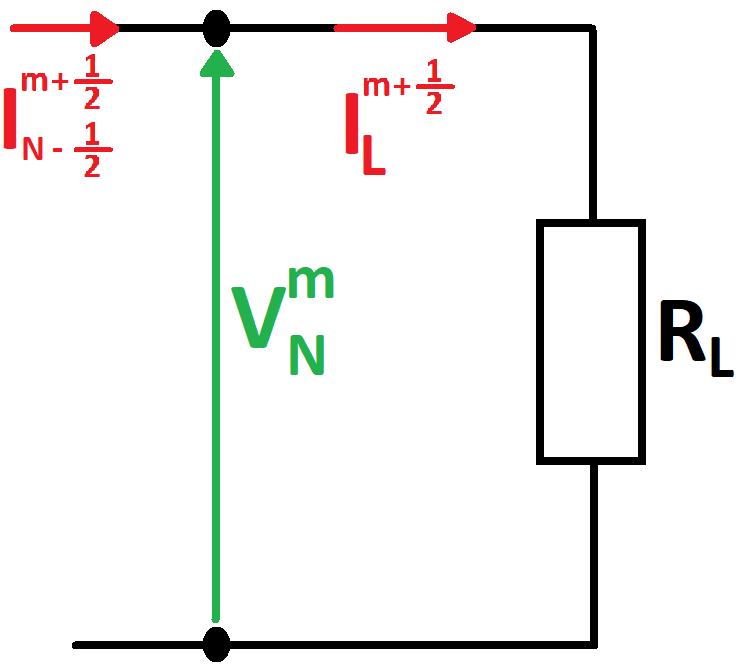
\includegraphics[scale=0.25]{BC2}
    \caption{Boundary situation at the $z=d$}
    \label{fig:Rl}
\end{figure}

The voltage update equation becomes:
\begin{equation}
    V^{m+1}_{N} = V^{m}_{N} + \frac{2\Delta t}{C\Delta z}\left(I^{m+\frac{1}{2}}_{N-\frac{1}{2}} - I^{m+\frac{1}{2}}_{L}\right)
    \label{BC2}
\end{equation}
Kirchoff's voltage law in discretized form states that
\begin{align}
    I^{m+\frac{1}{2}}_{L} & = \frac{V^{m+\frac{1}{2}}_{N}}{R_{L}}\nonumber\\
    & = \frac{V^{m}_{N}+V^{m+1}_{N}}{2R_{L}}
    \label{IL}
\end{align}
Subsituting (\ref{IL}) in (\ref{BC2}) and using the same relations as for $z=0$ yields, 
after some rearrangements:
\begin{equation}
    V^{m+1}_{N} = K_{2}V^{m}_N + 2\kappa_{2}\tilde{I}^{m+\frac{1}{2}}_{N-\frac{1}{2}},
\end{equation}
where
\begin{align}
    K_{2} & = \frac{R_{L}-\alpha R_{c}}{R_{L}+\alpha R_{c}},\\
    \kappa_{2} & = \frac{\alpha R_{c}}{R_{L}+\alpha R_{c}},
\end{align}
are two dimensionless constants which also will be discussed in a following section.